\documentclass[12pt,a4paper]{article}

% Packages
\usepackage[utf8]{inputenc}
\usepackage[T1]{fontenc}
\usepackage{amsmath}
\usepackage{amsfonts}
\usepackage{amssymb}
\usepackage{graphicx}
\usepackage{float}
\usepackage{listings}
\usepackage{xcolor}
\usepackage{hyperref}
\usepackage{geometry}
\usepackage{cite}
\usepackage{enumitem}
\usepackage{subcaption}
\usepackage{booktabs}
\usepackage{tikz}
\usetikzlibrary{trees, arrows.meta, positioning, automata}
\usepackage{dirtree}


% Page setup
\geometry{margin=1in}

% Code listing style
\lstset{
    basicstyle=\ttfamily\small,
    breaklines=true,
    frame=single,
    numbers=left,
    numberstyle=\tiny,
    keywordstyle=\color{blue},
    commentstyle=\color{green},
    stringstyle=\color{red}
}

% Title information
\title{FPGA-Based Zombie Shooting Game with VGA Display and Audio System}
\author{Your Name}
\date{\today}

\begin{document}

% Title page
\maketitle
\thispagestyle{empty}
\newpage

% Table of contents
\tableofcontents
\newpage

% ============================================
% File Structure
% ============================================
\section{File Structure}

\dirtree{%
.1 team06\_final/.
.2 team06\_final\_report.pdf.
.2 team06\_final\_presentation.pdf.
.2 src/.
.3 DE2\_115/.
.4 DE2\_115.sv.
.4 DE2\_115.sdc.
.4 DE2\_115.qsf.
.3 IMU/.
.4 uart\_rx.sv.
.4 imu\_parser.sv.
.4 velocity\_integrator.sv.
.3 zombie\_position\_control/.
.4 Position\_Controller.sv.
.4 Random\_Position\_Generator.sv.
.3 Audio/.
.4 audio\_control.sv.
.4 AudPlayer.sv.
.4 I2cInitializer.sv.
.3 VGA\_720p/.
.4 VGA\_Controller\_720p.sv.
.4 VGA\_Compositor\_720p.sv.
.3 others/.
.4 Debounce.sv.
.4 HexTo7Seg.sv.
.4 Start\_Game\_Detector.sv.
.2 BRAMs/.
.3 aim/.
.4 aim.qip, aim.v, aim sprite data.
.3 audio/.
.4 bgm.mif, killed.mif, BGM and sound effects.
.3 background/.
.4 background\_palette.v, start\_palette.v.
.3 end/.
.4 win\_palette.v, lose\_palette.v, retry\_palette.v.
.3 zombies/.
.4 zombie\_05x.v, zombie\_06x.v, zombie\_07x.v, zombie\_08x.v, zombie\_09x.v, zombie\_1x.v.
.4 zombie\_*x\_bound.v, zombie\_*x\_bound2.v (transparency bounds).
.4 zombie\_1x\_palette.v (used by every zombies).
}

% ============================================
% 1. Topic
% ============================================
\section{Topic}

This project presents a fully functional, real-time zombie shooting game implemented entirely on an FPGA platform. The system delivers an immersive gaming experience through high-definition 720p VGA graphics, dynamic audio feedback, and intuitive motion-based aiming control using an Inertial Measurement Unit (IMU). Players engage in an action-packed survival scenario where they must eliminate waves of zombies approaching from various positions on screen, with the game dynamically adjusting difficulty based on performance.

The core innovation lies in the seamless integration of multiple complex subsystems operating in parallel: a pixel-perfect VGA display engine capable of rendering multiple animated sprites simultaneously, a sophisticated audio playback system providing background music and sound effects, and a responsive motion control interface that translates physical movements into precise on-screen aiming. The game features intelligent zombie spawning algorithms, real-time collision detection, dynamic sprite scaling for depth perception, and comprehensive game state management including win/lose conditions and scoring mechanisms.

\subsection{Key Advantages}

The FPGA-based implementation offers several significant advantages over traditional software-based game systems:

\begin{itemize}
    \item \textbf{Ultra-Low Latency}: Hardware-accelerated rendering and processing eliminate software overhead, providing near-instantaneous response to player inputs. The parallel architecture ensures that VGA timing, audio playback, and game logic execute simultaneously without interference.
    
    \item \textbf{Real-Time Performance}: The dedicated hardware pipeline guarantees consistent 60 frames per second rendering at 1280x720 resolution, with deterministic timing for all game mechanics. Unlike software implementations that may suffer from frame drops or timing jitter, this system maintains precise synchronization across all subsystems.
    
    \item \textbf{Memory Efficiency}: By utilizing palette-based color indexing and strategic use of SRAM for large background images and BRAM for frequently accessed sprite data, the system achieves high-quality graphics while minimizing memory footprint. Multiple zombie sprites at different scales are stored efficiently, enabling up to 20 simultaneous zombies on screen.
    
    \item \textbf{Deterministic Behavior}: All game logic executes in fixed clock cycles, ensuring predictable and reproducible gameplay. This determinism is crucial for game mechanics such as collision detection, zombie movement patterns, and audio synchronization.
    
    \item \textbf{Modular Architecture}: The system is designed with clear module boundaries, making it easy to modify, extend, or debug individual components. Each subsystem (VGA, audio, input control, game logic) operates independently while communicating through well-defined interfaces.
    
    \item \textbf{Power Efficiency}: FPGA implementations can be more power-efficient than general-purpose processors for dedicated tasks, as only the required logic is active, and there is no instruction fetch overhead.
    
    \item \textbf{Educational Value}: This project demonstrates practical application of digital design principles including state machines, pipeline architectures, memory interfaces, clock domain crossing, and real-time system design.
\end{itemize}

The system successfully demonstrates that complex, interactive multimedia applications can be efficiently implemented on FPGA platforms, providing a foundation for future embedded gaming systems, interactive displays, or real-time graphics applications.

% ============================================
% 2. Overview
% ============================================
\section{Overview}
% TODO: Write overview of the project

This project, titled "FPGA-Based Zombie Shooting Game", is a real-time interactive survival game that leverages the high-performance parallel processing capabilities of FPGAs. The game tasks players with defending against waves of zombies using an IMU-based motion control system. By combining high-definition VGA graphics, synchronized audio effects, and low-latency input processing, the system provides a compelling demonstration of complex system-on-chip (SoC) design on an FPGA.

\subsection{System Architecture}
% TODO: Write system architecture overview

The system follows a modular architecture where the top-level module (\texttt{DE2\_115}) orchestrates the communication between several key functional blocks. This modularity ensures efficient data flow and clear separation of concerns:

\begin{itemize}
    \item \textbf{Display Subsystem}: Centered around the \texttt{VGA\_Controller\_\allowbreak 720p} and \texttt{VGA\_Image\_\allowbreak Overlay\_Combined} modules. It manages a 6-stage pipeline to composite multiple layers (background, sprites, and UI) in real-time.
    \item \textbf{Input Subsystem}: Processes motion data from an external \textbf{LSM6DSL IMU} mounted on an \textbf{STM32L4S5VIT6} microcontroller. The STM32 reads raw sensor data via I2C and transmits orientation information to the FPGA through UART. A \texttt{UART\_RX} module on the FPGA receives this data, which is then parsed by the \texttt{IMU\_Parser} and integrated by the \texttt{Position\_Controller} to drive the on-screen aim cursor.
    \item \textbf{Audio Subsystem}: Managed by the \texttt{audio\_control} module, it handles background music (BGM) playback and triggers specific sound effects (SFX) for game events like shooting or zombie deaths.
    \item \textbf{Game Logic}: Implements the core mechanics, including random zombie spawning (\texttt{Random\_Position\_Generator}), collision detection (within the compositor), life tracking, and win/lose condition management.
    \item \textbf{Memory Hierarchy}: Balanced use of External SRAM (for high-resolution backgrounds) and On-chip BRAM (for localized sprite indices, palettes, and transparency bounds).
\end{itemize}

\subsection{Hardware Platform}
% TODO: Write hardware platform (DE2-115)

The system is developed and deployed on the \textbf{Terasic DE2-115 Development Board}, featuring a Cyclone IV EP4CE115 FPGA. The following hardware resources and peripherals are utilized:

\begin{itemize}
    \item \textbf{Cyclone IV FPGA}: The heart of the system, implementing all logic and on-chip memory.
    \item \textbf{2MB SRAM}: Used as a frame buffer and storage for large indexed images (1280x720).
    \item \textbf{VGA (ADV7123)}: High-speed video DAC driving the 720p (74.25MHz) display output.
    \item \textbf{Audio Codec (WM8731)}: Provides high-quality audio output for game music and effects.
    \item \textbf{LSM6DSL IMU}: A 6-axis motion tracking device (accelerometer and gyroscope) used for orientation sensing.
    \item \textbf{STM32 L4S5VIT6}: Acts as an intelligent sensor hub, performing initial data acquisition from the IMU and bridging it to the FPGA via UART.
    \item \textbf{GPIO \& Buttons}: Used for trigger inputs (shooting), hardware resets, and diagnostic controls.
\end{itemize}

\subsection{Main Features}
% TODO: Write main features

Key features of the implementation include:

\begin{itemize}
    \item \textbf{720p Real-Time Graphics}: Crisp 1280x720 resolution rendered at a consistent 60 FPS without software-related jitter.
    \item \textbf{3D Depth Perception}: Dynamic scaling of zombie sprites (from 0.5x to 1.0x) based on their vertical position, simulating a 3D environment.
    \item \textbf{Responsive Motion Aiming}: Low-latency translation of IMU orientation to target coordinates, providing a "light-gun" style experience.
    \item \textbf{Multi-Sprite Rendering}: Capability to render up to 20 independent zombies simultaneously with individual states and animations.
    \item \textbf{Interactive Audio}: Seamless blending of background survival-themed music with real-time sound effects for shooting and zombie eliminations.
    \item \textbf{Robust Game States}: Integrated flow from a start screen to active gameplay, including difficulty scaling and terminal win/lose states.
\end{itemize}

% ============================================
% 3. Methods
% ============================================
\section{Methods}

This section describes the key algorithms and memory management techniques employed in the system to achieve efficient image processing and rendering.

\subsection{Algorithms}

\subsubsection{K-means Color Quantization}
The system uses K-means clustering algorithm to reduce the color space of source images from 24-bit RGB (16.7 million colors) to 8-bit indexed color (256 colors). This compression technique is essential for fitting large images into limited FPGA memory resources while maintaining acceptable visual quality.

\paragraph{Algorithm Overview}
The K-means quantization process works as follows:
\begin{enumerate}
    \item \textbf{Image Preprocessing}: Source images are loaded in RGBA format, where the alpha channel (A) is used to identify transparent pixels.
    \item \textbf{Transparent Pixel Handling}: All pixels with alpha channel value of 0 are automatically assigned index 0, which maps to white (255, 255, 255) in the palette. This white color serves as the transparent key.
    \item \textbf{Cluster Initialization}: The algorithm creates K-1 clusters (where K=256) from all non-transparent pixels. The remaining cluster (index 0) is reserved for transparency.
    \item \textbf{K-means Clustering}: The scikit-learn KMeans algorithm is applied to the RGB values of all opaque pixels, finding optimal cluster centers that minimize the sum of squared distances from pixels to their nearest cluster center.
    \item \textbf{White Color Avoidance}: If any cluster center results in pure white (255, 255, 255), it is automatically adjusted to (254, 254, 254) to avoid conflicts with the transparency key.
    \item \textbf{Index Assignment}: Each pixel is assigned to its nearest cluster center using Euclidean distance in RGB space:
    \begin{equation}
    \text{distance} = \sqrt{(R - R_c)^2 + (G - G_c)^2 + (B - B_c)^2}
    \end{equation}
    where $(R_c, G_c, B_c)$ are the cluster center coordinates.
    \item \textbf{Palette Generation}: The final palette consists of 256 entries: index 0 = white (transparent), indices 1-255 = K-means cluster centers converted to RGB565 format.
\end{enumerate}

\paragraph{RGB565 Conversion}
The palette colors are stored in RGB565 format (16 bits) to match the BRAM data width:
\begin{equation}
\text{RGB565} = (R \gg 3) \ll 11 \mid (G \gg 2) \ll 5 \mid (B \gg 3)
\end{equation}
This format allocates 5 bits for red, 6 bits for green, and 5 bits for blue, providing a good balance between color accuracy and memory efficiency.

\paragraph{Output Format}
The quantization process generates three types of output files:
\begin{itemize}
    \item \textbf{Index Map (.bin/.mif)}: Binary file containing 8-bit pixel indices, stored row by row
    \item \textbf{Palette File (.mif)}: Memory initialization file containing 256 RGB565 color values
    \item \textbf{Preview Image (.png)}: Reconstructed image for visual verification
\end{itemize}

\subsubsection{Image Overlay with Bounds Checking}
To properly composite multiple image layers (background, zombies, aim cursor) without artifacts, the system implements sophisticated bounds checking and transparency handling.

\paragraph{Bounds Calculation}
For each sprite (zombie), the system pre-computes transparency bounds to optimize rendering performance. The bounds calculation algorithm:
\begin{enumerate}
    \item \textbf{Column-wise Scanning}: For each column (X coordinate) in the sprite, the algorithm scans from top to bottom (Y coordinate).
    \item \textbf{Min/Max Detection}: For each column, it finds:
    \begin{itemize}
        \item \textbf{Min Y}: The first (topmost) non-transparent pixel (index $\neq$ 0)
        \item \textbf{Max Y}: The last (bottommost) non-transparent pixel (index $\neq$ 0)
    \end{itemize}
    \item \textbf{Bounds Storage}: The result is stored as a 16-bit value per column: [15:8] = Max Y, [7:0] = Min Y
    \item \textbf{Full Transparent Columns}: If a column contains only transparent pixels, Min Y = 0xFF and Max Y = 0x00, indicating the entire column should be skipped
\end{enumerate}

\paragraph{Overlay Rendering Algorithm}
The image compositor uses a multi-stage pipeline to determine the final pixel color:
\begin{enumerate}
    \item \textbf{Stage 0 - Candidate Selection}: For each pixel coordinate (h\_count, v\_count), determine which sprites might overlap this position based on their bounding boxes.
    \item \textbf{Stage 1 - Bounds Check}: For each candidate sprite, check if the current pixel is within the sprite's bounds and within the non-transparent region (using pre-computed bounds).
    \item \textbf{Stage 2 - Priority Resolution}: If multiple sprites overlap the same pixel, determine rendering priority (typically: aim cursor > zombies > background).
    \item \textbf{Stage 3 - Pixel Index Fetch}: Read the pixel index from the appropriate memory (SRAM for background, BRAM for sprites).
    \item \textbf{Stage 4 - Palette Lookup}: Convert the 8-bit index to RGB565 color using the palette BRAM.
    \item \textbf{Stage 5 - RGB Conversion}: Convert RGB565 to RGB888 for VGA output, applying any special effects (hit flash, grayscale for dying zombies).
\end{enumerate}

\paragraph{Transparency Handling}
Transparent pixels (index = 0x00) are handled by:
\begin{itemize}
    \item Skipping palette lookup for transparent pixels
    \item Falling through to the next layer (background) when a sprite pixel is transparent
    \item Using bounds information to avoid unnecessary memory accesses for fully transparent regions
\end{itemize}

\subsection{Memory Management}

\subsubsection{Index-Based Storage}
The system uses an 8-bit index-based storage scheme to minimize memory requirements:
\begin{itemize}
    \item \textbf{Background Images}: Stored in external SRAM as 8-bit indices (1 byte per pixel)
    \item \textbf{Sprite Images}: Stored in BRAM as 8-bit indices (1 byte per pixel)
    \item \textbf{Memory Savings}: A 1280×720 image requires only 921,600 bytes (900 KB) instead of 2,764,800 bytes (2.7 MB) for 24-bit RGB
    \item \textbf{Address Calculation}: Pixel address = Y × WIDTH + X, stored in row-major order
\end{itemize}

\subsubsection{Palette System}
The palette system provides color lookup for indexed images:
\begin{itemize}
    \item \textbf{Palette Storage}: Each palette is stored in BRAM as 256 entries of 16-bit RGB565 values
    \item \textbf{Memory Layout}: Palette BRAM address = pixel index (0-255), data = RGB565 color value
    \item \textbf{Multiple Palettes}: Different palettes are used for different image types:
    \begin{itemize}
        \item Background palette: For start screen and game background
        \item Zombie palette: For zombie sprites at different scales
        \item End game palettes: For win/lose/retry screens
    \end{itemize}
    \item \textbf{Palette Lookup}: The conversion from index to color is a single-cycle BRAM read operation
\end{itemize}

\subsubsection{Bounds Management}
To optimize rendering performance, the system maintains bounds information for sprites:
\begin{itemize}
    \item \textbf{Pre-computed Bounds}: Transparency bounds are calculated once per sprite and stored in registers
    \item \textbf{Bounds Format}: For each X coordinate, bounds store [Max Y, Min Y] as a 16-bit value
    \item \textbf{Bounds Usage}: During rendering, bounds are checked before accessing sprite pixel data:
    \begin{itemize}
        \item If current Y < Min Y or Y > Max Y: Skip sprite pixel fetch (column is transparent at this Y)
        \item If Min Y $\le$ Y $\le$ Max Y: Fetch sprite pixel and check if index = 0 (pixel-level transparency)
    \end{itemize}
    \item \textbf{Performance Benefit}: Bounds checking eliminates unnecessary memory accesses for transparent regions, reducing memory bandwidth and improving timing closure
\end{itemize}

\subsubsection{Memory Hierarchy}
The system employs a hierarchical memory architecture optimized for different access patterns:
\begin{itemize}
    \item \textbf{SRAM (External)}: 
    \begin{itemize}
        \item Capacity: 2MB (1M × 16-bit words)
        \item Usage: Large background images (1280×720 = 921,600 bytes)
        \item Access: Sequential, predictable pattern (row-by-row scanning)
        \item Latency: 2 clock cycles
    \end{itemize}
    \item \textbf{BRAM (On-chip)}:
    \begin{itemize}
        \item Capacity: Multiple 256×8-bit blocks for sprites, 256×16-bit blocks for palettes
        \item Usage: Frequently accessed sprite data and palette lookups
        \item Access: Random access for sprite rendering
        \item Latency: 1 clock cycle
    \end{itemize}
    \item \textbf{Register Arrays}:
    \begin{itemize}
        \item Usage: Bounds information, game state, zombie positions
        \item Access: Immediate (combinational)
        \item Latency: 0 cycles (combinational logic)
    \end{itemize}
\end{itemize}

\subsubsection{Address Mapping}
The system uses different address mapping strategies for different memory types:
\begin{itemize}
    \item \textbf{SRAM Address}: 
    \begin{equation}
    \text{SRAM\_ADDR} = \text{Y} \times \text{WIDTH} + \text{X}
    \end{equation}
    Since SRAM is 16-bit wide, byte address is divided by 2, and the lower bit selects high/low byte.
    \item \textbf{BRAM Address (Sprites)}:
    \begin{equation}
    \text{BRAM\_ADDR} = (\text{Y} - \text{sprite\_y}) \times \text{sprite\_width} + (\text{X} - \text{sprite\_x})
    \end{equation}
    where sprite coordinates are relative to the sprite's top-left corner.
    \item \textbf{BRAM Address (Palette)}:
    \begin{equation}
    \text{Palette\_ADDR} = \text{pixel\_index}
    \end{equation}
    Direct mapping from pixel index to palette entry.
\end{itemize}

% ============================================
% 4. Module Introduction
% ============================================
\section{Module Introduction}

\subsection{VGA Display Modules}
\subsubsection{VGA Controller 720p}

\paragraph{Module Goals}
The VGA Controller 720p generates timing signals for 1280x720@60Hz VGA output at 74.25MHz. It produces sync, blanking signals, and pixel coordinates with a 5-cycle delay pipeline to compensate for BRAM latency.

\paragraph{Detailed Description}

The VGA Controller 720p module implements a complete VGA timing generator conforming to the VESA standard for 1280x720@60Hz (720p) resolution. This module serves as the foundation of the display system, providing all necessary timing signals and pixel coordinate information to downstream rendering modules.

\paragraph{Timing Parameters}
The module implements the standard 720p timing parameters as defined in the VESA specification:
\begin{itemize}
    \item \textbf{Horizontal Timing}: Total line length of 1650 pixels, consisting of 1280 active display pixels, 110 front porch, 40 sync pulse, and 220 back porch pixels
    \item \textbf{Vertical Timing}: Total frame length of 750 lines, consisting of 720 active display lines, 5 front porch, 5 sync pulse, and 20 back porch lines
    \item \textbf{Clock Frequency}: 74.25MHz, generated by a PLL from the 50MHz system clock
    \item \textbf{Refresh Rate}: 60Hz, calculated as 74.25MHz / (1650 × 750) = 60.0 Hz
\end{itemize}

\paragraph{Architecture and Design}
The module employs a clean separation between combinational logic (denoted with `\_w` suffix for "write" values) and sequential logic (denoted with `\_r` suffix for "register" values). This design pattern improves code readability and facilitates timing analysis.

The core functionality consists of two main counters:
\begin{itemize}
    \item \textbf{Horizontal Counter (h\_count\_r)}: Counts from 0 to 1649 (H\_TOTAL - 1), incrementing every clock cycle
    \item \textbf{Vertical Counter (v\_count\_r)}: Counts from 0 to 749 (V\_TOTAL - 1), incrementing when the horizontal counter wraps around
\end{itemize}

\paragraph{BRAM Delay Compensation}
A critical feature of this controller is its ability to compensate for BRAM read latency. The module calculates active pixel coordinates one cycle ahead of when they are actually needed. Specifically:
\begin{itemize}
    \item At cycle T, the module calculates the active coordinates (h\_active\_count\_w, v\_active\_count\_w) based on the current counter values (h\_count\_r, v\_count\_r)
    \item These calculated coordinates are registered in the next cycle (T+1) as h\_active\_count\_r and v\_active\_count\_r
    \item These registered coordinates are then output as o\_h\_count and o\_v\_count, which are used by the VGA Image Compositor to fetch pixel data
    \item This 1-cycle advance compensates for the 1-cycle read latency of BRAM, ensuring pixel data arrives at the correct time for display
\end{itemize}

The active coordinate calculation logic checks if the current position is within the active display region:
\begin{align}
\text{h\_active\_count\_w} &= \begin{cases}
\text{h\_count\_r} - \text{H\_BACK\_PORCH} & \text{if } \text{H\_BACK\_PORCH} \leq \text{h\_count\_r} < \text{H\_BACK\_PORCH} + \text{H\_DISPLAY} \\
0 & \text{otherwise}
\end{cases}
\end{align}

\paragraph{Signal Generation}
The module generates all standard VGA timing signals:
\begin{itemize}
    \item \textbf{HSYNC (o\_hsync)}: Horizontal synchronization pulse, active low during the sync period (pixels 1610-1649)
    \item \textbf{VSYNC (o\_vsync)}: Vertical synchronization pulse, active low during the sync period (lines 745-749)
    \item \textbf{BLANK\_N (o\_blank\_n)}: Active high during the visible display region, low during blanking periods
    \item \textbf{SYNC\_N (o\_sync\_n)}: Always low for standard VGA operation
    \item \textbf{VGA\_CLK (o\_vga\_clk)}: Pass-through of the 74.25MHz clock to the VGA connector
\end{itemize}

\paragraph{5-Cycle Delay Pipeline}
To ensure proper synchronization with downstream processing stages, the module implements a 5-cycle delay pipeline for all output signals. This pipeline:
\begin{itemize}
    \item Delays HSYNC, VSYNC, BLANK\_N, SYNC\_N, and active\_video signals by 5 clock cycles
    \item Delays h\_count and v\_count coordinate outputs by 5 clock cycles
    \item Ensures that timing signals and pixel coordinates remain synchronized even after multiple pipeline stages in the image compositor
\end{itemize}

The pipeline uses shift registers to implement the delay:
\begin{lstlisting}[language=Verilog, basicstyle=\ttfamily\small]
hsync_delay <= {hsync_delay[3:0], hsync_int};
vsync_delay <= {vsync_delay[3:0], vsync_int};
// ... similar for other signals
\end{lstlisting}

\paragraph{Output Signals}
The module provides the following outputs to the VGA Image Compositor:
\begin{itemize}
    \item \textbf{o\_h\_count [10:0]}: Horizontal pixel coordinate (0-1279) within the active display region
    \item \textbf{o\_v\_count [9:0]}: Vertical pixel coordinate (0-719) within the active display region
    \item \textbf{o\_active\_video}: High when the current pixel position is within the active display region
\end{itemize}

These outputs are used by the VGA Image Compositor to determine which pixel data to fetch from SRAM (for background) and BRAM (for sprites), ensuring that the correct image data is displayed at each pixel position.

\paragraph{Reset Behavior}
Upon reset (i\_rst\_n = 0), all counters and delay pipeline registers are initialized to zero, placing the controller in a known state at the beginning of a frame. The module immediately begins generating valid timing signals after reset is released.

\subsubsection{VGA Image Compositor}
\paragraph{Module Goals}
The VGA Image Compositor is the core rendering engine that composites multiple image layers (background, up to 20 zombie sprites, aim cursor, and end-game screens) into a single RGB output stream. It implements a 6-stage pipeline architecture with sprite scaling (0.5x to 1.0x), transparency handling, collision detection, and visual effects. The module manages SRAM and BRAM interfaces with different access latencies and uses bounds checking to optimize rendering performance.

\paragraph{Detailed Description}
The VGA Image Compositor is a sophisticated 6-stage pipelined rendering engine that composites multiple image layers in real-time. It handles background images from SRAM, up to 20 zombie sprites from BRAM, an aim cursor overlay, and end-game screens, producing a single RGB888 output stream at 74.25MHz.

\paragraph{Architecture Overview}
The module implements a 6-stage pipeline architecture optimized for memory latency compensation:
\begin{itemize}
    \item \textbf{Layer 0}: Candidate Selection \& Address Calculation (Combinational)
    \item \textbf{Layer 1}: Memory Request \& SRAM Address Output
    \item \textbf{Layer 2}: Bounds Check \& ID Select \& SRAM Data Latch
    \item \textbf{Layer 3}: Pixel Index Fetch (BRAM \& SRAM Parse)
    \item \textbf{Layer 4}: Palette Fetch
    \item \textbf{Layer 5}: RGB Conversion \& Mixing
\end{itemize}

\paragraph{Input Registration}
All inputs are registered in the first stage to improve timing closure and reduce combinational path delays. This includes pixel coordinates (h\_count, v\_count), zombie positions and valid flags, aim position, game state signals, and control signals.

\paragraph{Layer 0: Candidate Selection and Address Calculation}
This combinational stage performs several critical calculations in parallel:

\textbf{Background Address Calculation}: The module calculates SRAM addresses for background images based on the current pixel position. For the start screen, it uses a 4-bit per pixel format (4 pixels per 16-bit SRAM word), while the game uses 8-bit per pixel format (2 pixels per word). The base address switches between START\_BG\_ADDR (start screen) and 0 (game playing) based on the i\_started signal.

\textbf{Aim Cursor Calculation}: The aim cursor is a 200×200 pixel overlay centered at the aim position. The module converts center coordinates to top-left corner coordinates using signed arithmetic to handle off-screen positions, then calculates the local pixel address within the aim sprite.

\textbf{End Game Images}: When win or lose signals are active, the module calculates addresses for end-game images (survived, died, retry) stored in SRAM at predefined addresses. These images are positioned at fixed screen coordinates.

\textbf{Zombie Candidate Selection}: The module scans all MAX\_ZOMBIES (20) zombies and selects up to 4 candidates that overlap the current pixel position. For each candidate, it:
\begin{itemize}
    \item Determines sprite size based on Y position (0.5x to 1.0x scaling for depth perception)
    \item Calculates local coordinates within the sprite
    \item Stores the zombie index, local coordinates, size selector, and valid flag
\end{itemize}

\textbf{Kill Target Detection}: When the trigger is pressed (i\_killing), the module captures the aim center position. This position is later checked during rendering to detect zombie hits.

\paragraph{Layer 1: Memory Request and SRAM Address Output}
This stage initiates memory requests for all required data:

\textbf{Bounds BRAM Requests}: For each of the 4 zombie candidates, the module requests transparency bounds data from BRAM. Since zombies can be at 6 different scales (0.5x to 1.0x), the module maintains separate bounds BRAM instances for each scale. Dual-port BRAMs are used to fetch bounds for 2 candidates simultaneously, requiring 2 BRAM instances per scale (total 12 BRAM instances).

\textbf{Aim BRAM Request}: The aim cursor pixel data is requested from a dedicated BRAM instance.

\textbf{SRAM Address Output}: The calculated background or end-game image address is output to the SRAM interface. The module handles byte selection (LB\_N, UB\_N) based on whether the image uses 4-bit or 8-bit pixel format.

\paragraph{Layer 2: Bounds Check and Priority Selection}
This stage performs bounds checking and selects which sprite to render:

\textbf{Bounds Checking}: For each zombie candidate, the module checks if the current Y coordinate falls within the non-transparent region using the bounds data retrieved in Layer 1. The bounds data format is [15:8] = Max Y, [7:0] = Min Y for each X coordinate.

\textbf{Priority Selection}: Among all opaque zombies (those passing bounds check), the module selects the one with the lowest Y coordinate (backmost zombie) for rendering. This ensures proper depth ordering.

\textbf{Zombie Pixel Address Calculation}: For the selected zombie, the module calculates the pixel address within the sprite BRAM based on local coordinates and the sprite width (which varies with scale).

\textbf{Kill Detection}: If the current pixel position matches the captured kill target position and a zombie is present, a kill signal is generated. This triggers the zombie's death animation (grayscale flashing effect).

\textbf{SRAM Data Latch}: The SRAM data from Layer 1 (2-cycle latency) is latched for parsing in the next stage.

\paragraph{Layer 3: Pixel Index Fetch}
This stage retrieves pixel indices from memory:

\textbf{Zombie Pixel Fetch}: The selected zombie's pixel index is requested from the shared zombie sprite BRAM. The address and size selector are output to the top-level module, which routes the request to the appropriate BRAM instance (0.5x to 1.0x).

\textbf{SRAM Pixel Parsing}: The background pixel index is extracted from the latched SRAM data. For 8-bit mode, the module selects the appropriate byte based on the address LSB. For 4-bit mode (start screen), it extracts one of 4 nibbles from the 16-bit word.

\textbf{Aim Pixel Fetch}: The aim cursor pixel data (2-bit) is retrieved from the aim BRAM.

\paragraph{Layer 4: Palette Fetch}
This stage converts pixel indices to RGB565 colors:

\textbf{Palette Lookup}: Each pixel index (8-bit for background/zombies, 2-bit for aim) is used to address the corresponding palette BRAM. The module maintains separate palettes for:
\begin{itemize}
    \item Background (start screen and game)
    \item Zombies (shared across all scales)
    \item End-game images (survived, died, retry)
    \item Aim cursor
\end{itemize}

\textbf{Transparency Handling}: If a zombie pixel index is 0x00 (transparent), the palette lookup is skipped and the background color is used instead.

\paragraph{Layer 5: RGB Conversion and Mixing}
This final stage produces the RGB888 output:

\textbf{RGB565 to RGB888 Conversion}: Palette colors are stored in RGB565 format (16 bits). The module converts to RGB888 (24 bits) using bit replication:
\begin{itemize}
    \item Red: 5 bits → 8 bits: \{rgb565[15:11], rgb565[15:13]\}
    \item Green: 6 bits → 8 bits: \{rgb565[10:5], rgb565[10:9]\}
    \item Blue: 5 bits → 8 bits: \{rgb565[4:0], rgb565[4:2]\}
\end{itemize}

\textbf{Layer Compositing}: The module composites layers in priority order:
\begin{enumerate}
    \item End-game images (highest priority when active)
    \item Aim cursor (if within aim bounds and pixel is opaque)
    \item Zombies (if within sprite bounds and pixel is opaque)
    \item Background (lowest priority, always present)
\end{enumerate}

\textbf{Visual Effects}:
\begin{itemize}
    \item \textbf{Hit Flash}: When a zombie hits the player (i\_zombie\_hit), the entire screen flashes red for 0.2 seconds by increasing red channel intensity.
    \item \textbf{Dying Zombie Effect}: When a zombie is killed, it enters a flashing state for 0.5 seconds, alternating between grayscale and background every 0.05 seconds. Grayscale conversion uses the formula: gray = (R + G + B) / 3.
    \item \textbf{Kill Detection Output}: When a zombie is hit, the module outputs the zombie index (o\_kill\_idx) and a kill enable signal (o\_kill\_en) to the game logic.
\end{itemize}

\paragraph{Sprite Scaling System}
The module implements dynamic sprite scaling based on Y position to create depth perception:
\begin{itemize}
    \item Y < 345: 0.5x scale (51×75 pixels)
    \item Y < 420: 0.6x scale (61×90 pixels)
    \item Y < 495: 0.7x scale (70×103 pixels)
    \item Y < 570: 0.8x scale (80×118 pixels)
    \item Y < 645: 0.9x scale (90×132 pixels)
    \item Y $\ge$ 645: 1.0x scale (102×149 pixels)
\end{itemize}

Each scale has its own sprite BRAM and bounds BRAM instances, selected dynamically based on the zombie's Y position.

\paragraph{Memory Interface Management}
The module efficiently manages multiple memory interfaces:
\begin{itemize}
    \item \textbf{SRAM}: 2-cycle read latency, 16-bit data width, used for large background and end-game images
    \item \textbf{BRAM (Sprites)}: 1-cycle read latency, 8-bit data width, used for frequently accessed zombie sprites
    \item \textbf{BRAM (Palettes)}: 1-cycle read latency, 16-bit data width, used for color lookup tables
    \item \textbf{BRAM (Bounds)}: 1-cycle read latency, 16-bit data width, used for transparency bounds
\end{itemize}

The pipeline stages are carefully designed to account for these different latencies, ensuring all data arrives at the correct stage for compositing.

\subsection{Game Logic Modules}
\subsubsection{Start Game Detector}

\paragraph{Module Goals}
The Start Game Detector module detects when the game should begin by checking if the aim cursor is within a predefined start box area and the trigger button is pressed simultaneously. It outputs a latched "started" signal that remains high until reset, and includes clock domain synchronization for button inputs and an enable signal for conditional activation.

\paragraph{Detailed Description}
The Start Game Detector is a critical user interface component that manages the transition from the start screen to active gameplay. It implements a two-condition detection mechanism requiring both spatial positioning and user interaction, ensuring intentional game initiation.

\paragraph{Start Condition Detection}
The module requires three simultaneous conditions to be met before the game starts:
\begin{enumerate}
    \item \textbf{Aim Position Check}: The aim cursor (controlled by IMU) must be positioned within a predefined rectangular region on the screen. The start box boundaries are parameterized:
    \begin{itemize}
        \item Horizontal range: X coordinates between \texttt{START\_BOX\_X\_MIN} (494) and \texttt{START\_BOX\_X\_MAX} (778)
        \item Vertical range: Y coordinates between \texttt{START\_BOX\_Y\_MIN} (571) and \texttt{START\_BOX\_Y\_MAX} (630)
    \end{itemize}
    The bounds checking is implemented using combinational logic that compares the 11-bit aim X coordinate and 10-bit aim Y coordinate against the parameterized boundaries.
    \item \textbf{Trigger Button Press}: The debounced trigger button must generate a positive edge pulse (\texttt{i\_trigger\_posedge}), indicating the user has pulled the trigger.
    \item \textbf{Enable Signal}: The module must be enabled via the \texttt{i\_enable} input, allowing the system to conditionally activate or deactivate the start detection logic.
\end{enumerate}

The start condition is evaluated as:
\begin{equation}
\text{start\_condition\_met} = \text{i\_rst\_n} \land \text{i\_enable} \land \text{aim\_in\_start\_box} \land \text{i\_trigger\_posedge}
\end{equation}

\paragraph{Clock Domain Synchronization}
The module operates in the VGA clock domain (74.25MHz) to ensure synchronization with the rendering pipeline. To handle asynchronous button inputs safely, the module implements a three-stage synchronizer for the manual reset button (KEY[3]):
\begin{itemize}
    \item Three flip-flops (\texttt{key3\_sync1}, \texttt{key3\_sync2}, \texttt{key3\_sync3}) are cascaded to eliminate metastability
    \item Falling edge detection is performed by comparing \texttt{key3\_sync2} and \texttt{key3\_sync3} to generate a one-clock pulse when KEY[3] is pressed
    \item This synchronization ensures reliable button press detection even when the button signal originates from a different clock domain
\end{itemize}

\paragraph{Latching Mechanism}
The module implements a latching behavior for the started signal:
\begin{itemize}
    \item Once the start condition is met and \texttt{started\_internal} transitions from 0 to 1, it remains latched at 1
    \item The latch persists until an explicit reset occurs, either through the asynchronous reset (\texttt{i\_rst\_n}) or manual reset via KEY[3]
    \item This ensures the game remains in the "started" state even if the aim cursor moves outside the start box or the trigger is released
    \item The internal signal is registered through an output flip-flop (\texttt{started\_output}) before being presented as \texttt{o\_started}, providing an additional pipeline stage for timing closure
\end{itemize}

\paragraph{Reset Behavior}
The module supports multiple reset mechanisms:
\begin{itemize}
    \item \textbf{Asynchronous Reset}: The primary reset signal (\texttt{i\_rst\_n}) immediately clears the started state when asserted low
    \item \textbf{Manual Reset}: Pressing KEY[3] generates a synchronized pulse that resets the started state, allowing players to restart the game without a full system reset
    \item Both reset mechanisms ensure the module returns to a known initial state (not started)
\end{itemize}

\paragraph{Parameterization}
The start box boundaries are parameterized at module instantiation, allowing different regions to be defined for different purposes. In the top-level design, two instances are used:
\begin{itemize}
    \item \textbf{Start Game Detector}: Detects game initiation with bounds X: 494-778, Y: 571-630
    \item \textbf{Retry Button Detector}: Reuses the same module to detect retry button presses in end-game screens with bounds X: 500-780, Y: 400-553
\end{itemize}
This design reuse demonstrates the module's flexibility and reduces code duplication.

\subsubsection{Random Position Generator}
% TODO: Introduce Random Position Generator module

\paragraph{Module Goals}
The Random Position Generator module is responsible for the independent lifecycle management of up to 20 zombie entities. It handles their randomized spawning, continuous movement towards the player's position, and difficulty adjustment based on the player's performance (kill count).

\paragraph{LFSR-Based Randomness}
To ensure unpredictable spawning patterns without excessive hardware overhead, the module implements a 32-bit Linear Feedback Shift Register (LFSR). The LFSR uses the polynomial taps at positions 31, 21, 1, and 0 to generate a pseudo-random bitstream. This stream provides random X-coordinates for new zombies, while their Y-coordinate is fixed at an off-screen "horizon" to simulate arrival from the distance.

\paragraph{Bresenham-Based Movement}
The module implements a hardware-optimized version of the Bresenham line algorithm to handle movement. Instead of complex floating-point calculations, it uses an error accumulator strategy:
\begin{itemize}
    \item \textbf{Delta Calculation}: Computes the horizontal ($dx$) and vertical ($dy$) distance to the target position (typical target Y is the bottom of the screen).
    \item \textbf{Error Accumulation}: In each movement step, the minor axis coordinate is incremented only when the accumulated error exceeds a threshold of the major axis distance.
    \item \textbf{Fixed Steps}: Zombies move by a fixed \texttt{VELOCITY} parameter in each active clock cycle, ensuring smooth and consistent translation.
\end{itemize}

\paragraph{Dynamic Difficulty Scaling}
The system features an adaptive difficulty engine that monitors the \texttt{i\_kill\_count} input to adjust two primary parameters:
\begin{enumerate}
    \item \textbf{Generation Rate}: The interval between zombie spawns decreases as the kill count rises, increasing the density of enemies on screen. Rates range from 1.0Hz at the start to over 2.5Hz at high kill counts.
    \item \textbf{Movement Velocity}: The base movement frequency is scaled using a dynamic divider system. As the player advances, the internal update ticks occur more frequently, making zombies move faster towards the destination.
\end{enumerate}

\paragraph{Arrival and Collision Logic}
When a zombie reaches the target coordinates or is killed by the player, its slot is marked as invalid, and its internal state is reset to be recycled for the next random spawn. If a zombie arrives at the target without being killed, the \texttt{o\_hit} signal is asserted for one clock cycle, triggering the game's life deduction logic.

\subsection{Audio Modules}
\subsubsection{Audio Control}
% TODO: Introduce Audio Control module

\paragraph{Module Goals}
The \texttt{audio\_control} module acts as the central coordinator for the audio subsystem. Its primary responsibilities include the initial configuration of the hardware audio codec via I2C and the management of synchronized, multi-track audio playback (Background Music and Sound Effects).

\paragraph{I2C Initialization}
Upon system reset, the module enters the \texttt{AUD\_I2C\_INIT} state. It utilizes a sub-module, \texttt{I2cInitializer}, to send a sequence of configuration commands to the WM8731 codec at 100kHz. This setup includes setting the sampling rate, enabling the DAC, and configuring the data format. Once the \texttt{i2c\_finished} signal is asserted, the system transitions to active audio playback.

\paragraph{Audio State Machine and Priority Logic}
The core logic is implemented as a finite state machine (FSM) that manages the transition between different audio streams:
\begin{itemize}
    \item \textbf{AUD\_PLAY\_BGM}: The default state where survival-themed background music is read from a 117,520-sample BRAM and looped continuously.
    \item \textbf{AUD\_PLAY\_KILLED}: This state is triggered by a \texttt{kill\_en} signal from the VGA subsystem. When active, it interrupts the BGM and switches the BRAM addressing to play a shorter "killed" sound effect.
\end{itemize}
The priority logic ensures that sound effects (SFX) take precedence over the background music, providing immediate auditory feedback for in-game actions.

\paragraph{Cross-Domain Clock Synchronization}
The module successfully bridges three distinct clock domains:
\begin{itemize}
    \item \textbf{50MHz System Clock}: Drives the main control FSM and I2C operations.
    \item \textbf{12MHz Audio Clock}: Used for synchronous BRAM reading to match the codec's sampling frequency.
    \item \textbf{74.25MHz VGA Clock}: The source of the \texttt{kill\_en} signal, which is debounced and synchronized to the system domain to prevent metastable transitions.
\end{itemize}

\paragraph{Memory Management}
To minimize memory usage, the module uses a single unified address counter (\texttt{bram\_addr}) while applying offsets in the logic to select between the \texttt{bgm\_rom} and \texttt{killed\_rom}. The addressing logic handles the different sizes and starting points of each audio track, ensuring seamless transitions and loop-back behaviors.

\subsubsection{AudPlayer}
% TODO: Introduce AudPlayer module

\paragraph{Module Goals}
The \texttt{AudPlayer} module serves as the final stage of the audio pipeline, responsible for serializing 16-bit digital audio data into a bitstream compatible with the external WM8731 audio codec's Digital-to-Analog Converter (DAC).

\paragraph{I2S-Compatible Serialization}
The module implements a serialization logic similar to the I2S protocol. It operates on two primary clock signals provided by the audio codec:
\begin{itemize}
    \item \textbf{Bit Clock (\texttt{i\_bclk})}: Synchronizes the transmission of individual bits.
    \item \textbf{Left/Right Clock (\texttt{i\_daclrck})}: Indicates whether the current data frame belongs to the left or right audio channel.
\end{itemize}

\paragraph{Shift Register Implementation}
At the core of the module is a 16-bit shift register. The serialization process follows an MSB-first (Most Significant Bit first) pattern:
\begin{itemize}
    \item When a rising edge of \texttt{i\_daclrck} is detected (indicating the start of a new audio frame), the 16-bit audio sample from the DSP (\texttt{i\_dac\_data}) is parallel-loaded into the shift register.
    \item On each subsequent cycle of \texttt{i\_bclk}, the register contents are shifted left by one bit.
    \item The highest bit of the register (\texttt{shift\_reg[15]}) is continuously assigned to the \texttt{o\_aud\_dacdat} output, creating a serial bitstream for the codec.
\end{itemize}

\paragraph{Synchronization and Timing}
To ensure reliable data transmission, the module uses a bit counter to track the progress of each 16-bit frame. The use of the codec-supplied clocks ensures that the FPGA remains perfectly synchronized with the analog output timing requirements of the WM8731 chip, preventing audio artifacts such as pops or timing drift.

\subsection{Input Control Modules}
\subsubsection{UART Receiver}
% TODO: Introduce UART Receiver module

\paragraph{Module Goals}
The \texttt{uart\_rx} module is the primary interface for receiving motion data from the external STM32L4S5VIT6 microcontroller. It autonomously decodes the Universal Asynchronous Receiver-Transmitter (UART) serial bitstream into 8-bit data packets for processing by the IMU parser.

\paragraph{Oversampling and Sampling Strategy}
To ensure reliable communication at 115,200 baud, the module employs an oversampling strategy based on the 50MHz system clock. The \texttt{CLKS\_PER\_BIT} parameter (set to 434) defines the number of clock cycles per bit. The module samples the incoming serial line exactly at the $(CLKS\_PER\_BIT)/2$ point for the start bit and at every $CLKS\_PER\_BIT$ interval thereafter. This middle-of-bit sampling technique provides maximum noise immunity and compensates for potential baud rate mismatches.

\paragraph{Sequential State Machine Logic}
The receiver features a robust 5-state finite state machine (FSM) to handle the serial protocol:
\begin{itemize}
    \item \textbf{IDLE}: Monitors the line for a high-to-low transition (start bit).
    \item \textbf{RX\_START\_BIT}: Validates the start bit by checking for a persistent low level at the mid-point.
    \item \textbf{RX\_DATA\_BITS}: Serially shifts in 8 data bits at calculated intervals, storing them in a temporary register.
    \item \textbf{RX\_STOP\_BIT}: Ensures the line returns to a high state, indicating a valid end of the frame.
    \item \textbf{CLEANUP}: Asserts the data-valid (\texttt{o\_Rx\_DV}) signal for one clock cycle and resets for the next byte.
\end{itemize}

\paragraph{Metastability Protection}
Given that the incoming asynchronous signal (\texttt{i\_Rx\_Serial}) originates from a different clock domain, the module implements a double-stage synchronization register. By piping the raw input through two flip-flops (\texttt{r\_Rx\_Data\_R} and \texttt{r\_Rx\_Data}), the system effectively eliminates potential metastable states, ensuring stable operation within the FPGA's internal logic.

\subsubsection{IMU Parser}
% TODO: Introduce IMU Parser module

\paragraph{Module Goals}
The \texttt{imu\_parser} module is responsible for interpreting the stream of characters received from the UART interface. It serves as a translation layer that converts the human-readable ASCII representation of sensor data into structured 32-bit signed integers, which are then used for physical calculations in the game world.

\paragraph{Protocol and Communication Format}
To ensure data integrity, the system utilizes a proprietary yet simple framing protocol. Each data packet transmitted from the STM32 follows a specific format:
\begin{itemize}
    \item \textbf{Start Frame Marker}: Every packet begins with the character `\$', allowing the parser to synchronize with the start of a transmission even if bytes were dropped during the sequential read.
    \item \textbf{Data Fields}: The packet contains six comma-separated numeric values representing acceleration ($a_x, a_y, a_z$) and gyroscope ($g_x, g_y, g_z$) data.
    \item \textbf{Termination}: Packets are terminated by a Line Feed (LF) or Carriage Return (CR) character, signaling the parser to commit the parsed values to the output registers.
\end{itemize}

\paragraph{Hardware-Level ASCII-to-Integer Conversion}
The core of the parser is an efficient extraction logic that processes individual characters in real-time. For each digit character received (0--9), the module updates its \texttt{current\_val} register using the formula:
\[ \text{current\_val} = (\text{current\_val} \times 10) + (\text{char} - \text{'0'}) \]
This eliminates the need for complex string-to-int library calls. The module also tracks a sign bit (\texttt{is\_negative}) triggered by the '-' character, which is applied once a comma or terminator is encountered.

\paragraph{Parser State Machine}
The parsing logic is implemented as a three-state machine:
\begin{enumerate}
    \item \textbf{IDLE}: Waits for the `\$' character to begin a new packet.
    \item \textbf{READ\_NUM}: Collects digits and signs, performing the integer conversion until a separator (comma or newline) is found.
    \item \textbf{VALIDATE}: Upon receiving a terminater, the machine updates all six output registers simultaneously and asserts the \texttt{data\_ready} signal for one clock cycle, notifying the downstream position controller of fresh sensor data.
\end{enumerate}

\subsubsection{Velocity Integrator}
% TODO: Introduce Velocity Integrator module

\paragraph{Module Goals}
The \texttt{velocity\_integrator} module is responsible for the numerical processing of raw sensor data. It performs two critical functions: initial sensor calibration to remove environmental biases and gravity components, and the integration of linear acceleration into velocity vectors to provide smooth, reactive control signals for the game's aim cursor.

\paragraph{Self-Calibration Phase}
Upon system activation, the module enters a \texttt{ST\_CALIB} state for approximately 10 seconds. During this phase, it accumulates 2,048 samples for all six sensor axes. Once the count is reached, it calculates the arithmetic mean for each axis:
\[ \text{Offset} = \frac{1}{2048} \sum_{i=1}^{2048} \text{Sample}_i \]
This offset effectively captures the steady-state gravity vector and internal sensor bias, which are then subtracted from all subsequent readings to isolate "true" user-initiated motion.

\paragraph{Double-Precision Numerical Integration}
To mitigate the inherent accumulation of numerical errors (drift) in inertial sensing, the module utilizes high-precision 64-bit internal registers (\texttt{v\_acc\_x/y/z}) for velocity integration. The integration follows the basic kinematic equation:
\[ v_{new} = v_{old} + (a_{current} - \text{Offset}) \]
By using 64-bit accumulators, the system maintains significant bit depth, minimizing quantization errors that would otherwise cause the cursor to "slide" across the screen during static periods.

\paragraph{Intelligent Drift Management}
To further stabilize the control system, the module implements two software-hardware hybridized stabilization techniques:
\begin{itemize}
    \item \textbf{Dynamic Deadzone}: A configurable \texttt{THRESHOLD} is applied to the compensated acceleration. Values within this range are treated as noise and ignored, preventing "micro-crawling" when the sensor is stationary.
    \item \textbf{Smart Reset Timer}: The module monitors the stability of the input signals. If the acceleration remains within the deadzone for a continuous \texttt{STABILITY\_PERIOD} (approx. 0.2s), the velocity accumulators are automatically zeroed. This "leaky integrator" behavior ensures that any residual drift is periodically corrected without interrupting active user movement.
\end{itemize}

\paragraph{Output Data Path}
The final 32-bit velocity outputs (\texttt{vx, vy, vz}) and bias-compensated gyroscope data (\texttt{gx\_out, gy\_out, gz\_out}) are presented to the top-level system, providing a clean and stable kinematic representation of the user's hand gestures.

\subsubsection{Position Controller}
% TODO: Introduce Position Controller module

\paragraph{Module Goals}
The \texttt{Position\_Controller} module serves as the final link in the IMU-to-Display processing chain. It translates the processed angular velocity data into precise 2D screen coordinates, providing the user with a low-latency, intuitive aiming interface for the zombie shooting game.

\paragraph{Kinematic Mapping}
The module implements a specific mapping between 3D physical movement and 2D virtual space. Assuming the IMU is mounted along the gun barrel (+y axis):
\begin{itemize}
    \item \textbf{Yaw ($\omega_z$)}: Rotation around the vertical axis is mapped to the horizontal screen position (\texttt{o\_x}).
    \item \textbf{Pitch ($\omega_x$)}: Rotation around the horizontal right-axis is mapped to the vertical screen position (\texttt{o\_y}).
\end{itemize}
The roll component ($\omega_y$) is ignored, as it does not affect the targeting offset in a standard 2D projection.

\paragraph{Numerical Integration Formulae}
The cursor position is updated iteratively using a discrete integration scheme. At each update interval (determined by the \texttt{UPDATE\_DIVIDER} parameter), the position increments are calculated as follows:
\begin{align*}
    \Delta x &= (KX \times \omega_z) / 1000 \\
    \Delta y &= -(KY \times \omega_x) / 1000
\end{align*}
where $KX$ and $KY$ are sensitivity constants. The negative sign for $\Delta y$ compensates for the inverted nature of the screen coordinate system, where "upward" motion corresponds to a decreasing Y-value.

\paragraph{Sensitivity and Performance Scaling}
To allow for fine-tuned user experiences, the module uses 32-bit sensitivity parameters (\texttt{KX}, \texttt{KY}). These are scaled by 1,000 to permit integer-based arithmetic without losing precision, effectively representing fixed-point sensitivity coefficients. An internal clock divider (\texttt{update\_counter}) ensures that the position is updated at a consistent frequency (e.g., 1000Hz), decoupling cursor speed from the main system clock.

\paragraph{Boundary Clamping and Safety}
To prevent the cursor from migrating off-screen, the module implements hard clamping logic. After each integration step, the new coordinates are compared against the \texttt{SCREEN\_WIDTH} and \texttt{SCREEN\_HEIGHT} parameters. If a result exceeds these bounds, the output is truncated to the literal edge of the display:
\begin{verbatim}
    if (new_pos_x < 0) pos_x <= 0;
    else if (new_pos_x >= SCREEN_WIDTH) pos_x <= SCREEN_WIDTH - 1;
\end{verbatim}
This ensures a robust user experience where the aim remains trapped within the visible viewport.

\section{System Architecture}

This section presents the overall system architecture and detailed data flow of the FPGA-based zombie shooting game. The architecture is divided into three main layers: the user input layer, the FPGA processing layer, and the display output layer.

\subsection{Overall System Architecture}

Figure \ref{fig:data_path} illustrates the high-level system architecture, showing how user inputs from the IMU sensor and trigger button are processed by the FPGA to generate game visuals on the display screen.

\begin{figure}[H]
    \centering
    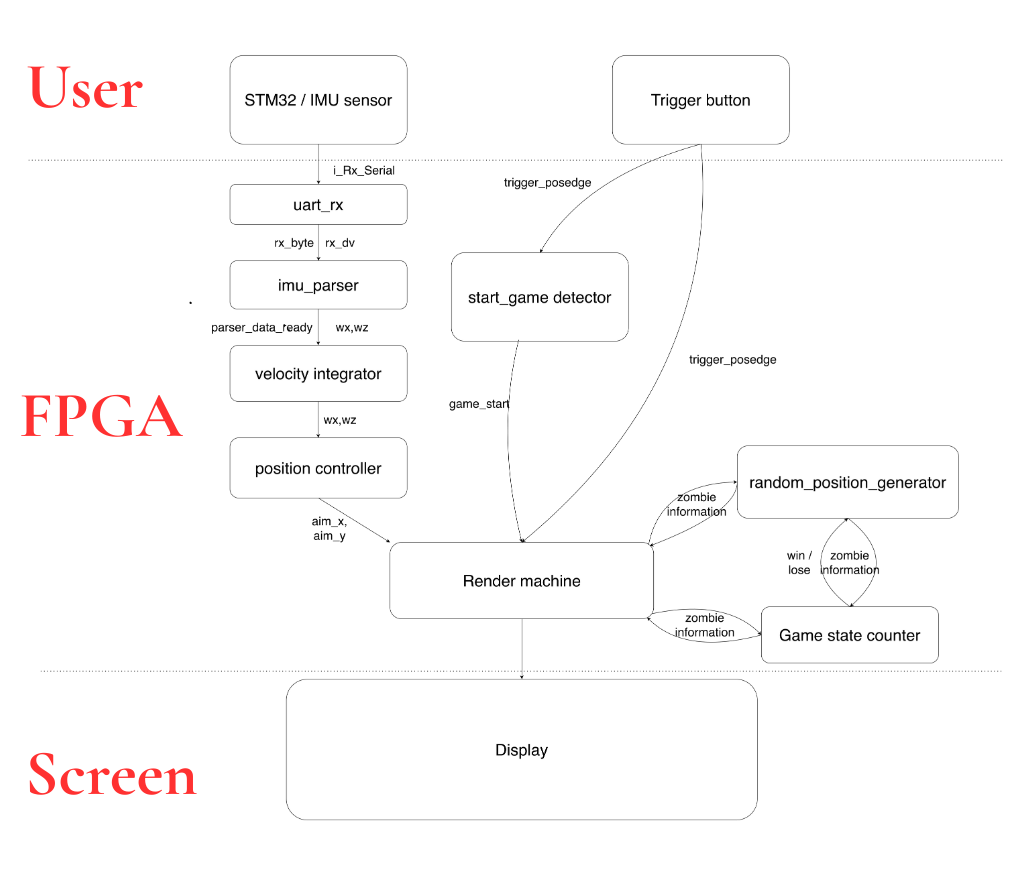
\includegraphics[width=0.95\textwidth]{data_path.png}
    \caption{Overall System Architecture and Data Flow}
    \label{fig:data_path}
\end{figure}

The architecture demonstrates the complete data path from user interaction to visual output:
\begin{itemize}
    \item \textbf{User Layer}: The STM32/IMU sensor provides motion data via UART, while the trigger button sends shooting commands directly to the FPGA.
    \item \textbf{FPGA Layer}: The central processing unit handles sensor data parsing, position calculation, game state management, random event generation, and rendering. Key components include the UART receiver, IMU parser, velocity integrator, position controller, game logic modules, and the render machine.
    \item \textbf{Screen Layer}: The final rendered output is displayed on the VGA monitor.
\end{itemize}

\subsection{Detailed Rendering Pipeline}

Figure \ref{fig:render_machine_detailed} shows the detailed architecture of the rendering subsystem, including clock generation, VGA controller, image compositor, and memory interfaces.

\begin{figure}[H]
    \centering
    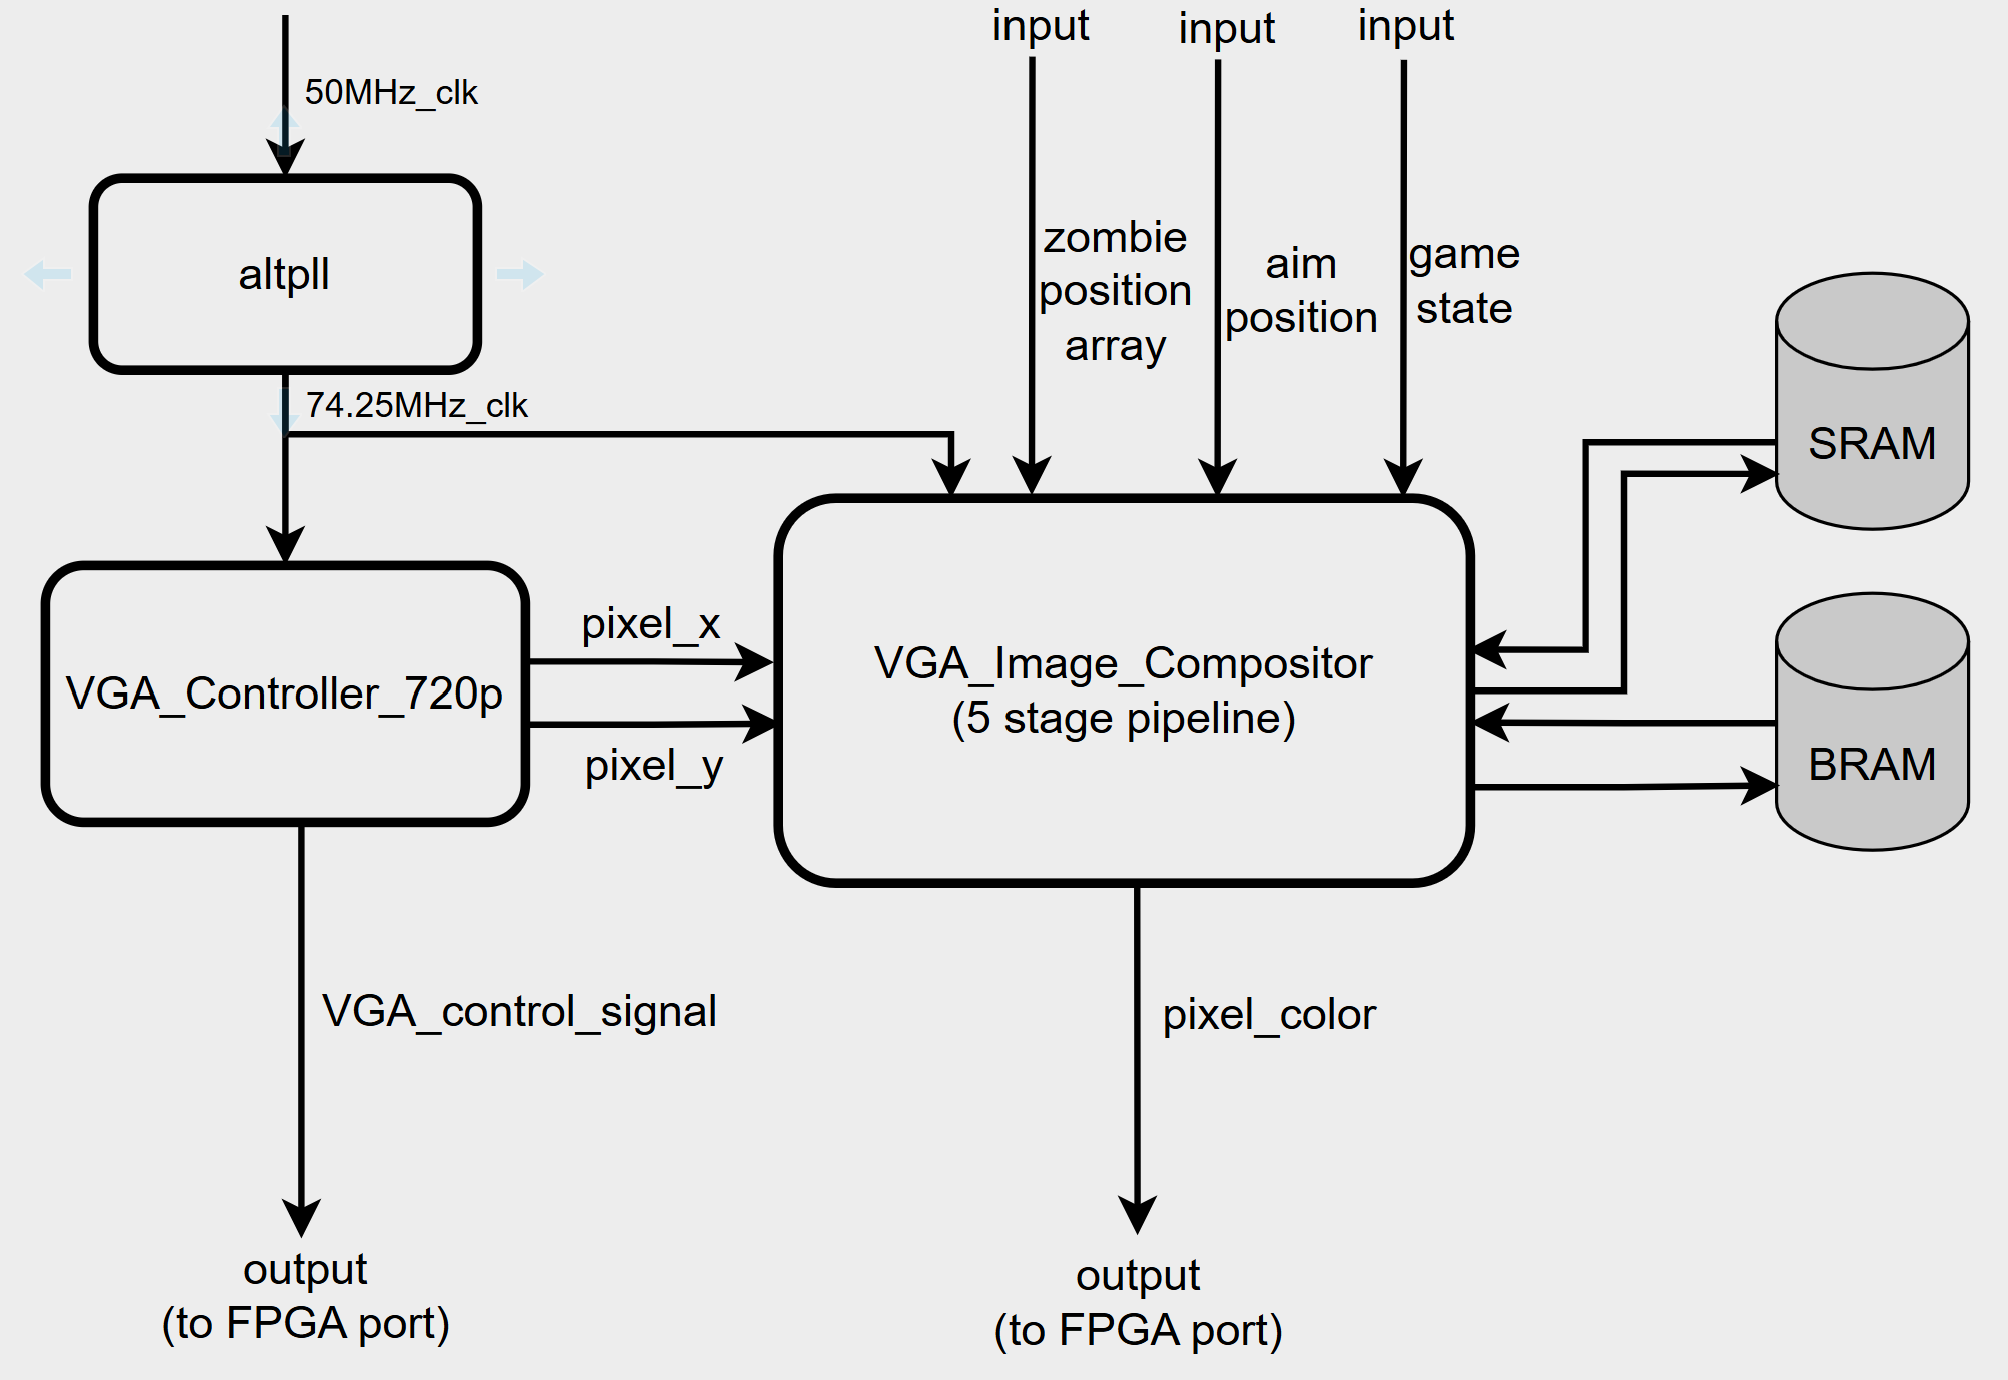
\includegraphics[width=0.95\textwidth]{render_machine_detailed.png}
    \caption{Detailed Rendering Pipeline Architecture}
    \label{fig:render_machine_detailed}
\end{figure}

The rendering pipeline consists of:
\begin{itemize}
    \item \textbf{Clock Generation}: The PLL generates a 74.25MHz clock from the 50MHz system clock to drive the VGA controller at 720p resolution.
    \item \textbf{VGA Controller}: Generates pixel coordinates (pixel\_x, pixel\_y) and VGA control signals for the display.
    \item \textbf{VGA Image Compositor}: A 5-stage pipelined architecture that composites multiple image layers (background, zombies, aim cursor) using game state information and zombie position arrays.
    \item \textbf{Memory Hierarchy}: The compositor interfaces with both external SRAM (for large background images) and on-chip BRAM (for sprite data and palettes) to efficiently manage memory resources.
\end{itemize}

\section{Finite State Machine (FSM) Diagrams}

% ---------- Common TikZ styles ----------
\tikzset{
    >=Stealth,
    fsmstate/.style={draw, rounded corners, align=center, minimum width=28mm, minimum height=8mm, font=\scriptsize},
    fsmarrow/.style={->, thick},
    fsmdashed/.style={->, thick, dashed},
    fsmerrow/.style={->, thick, bend right=18},
}

% =========================================================
% 1) Velocity Integrator FSM
% =========================================================
\begin{figure}[H]
\centering
\resizebox{0.95\textwidth}{!}{%
\begin{tikzpicture}[node distance=60mm]
    \node[fsmstate] (calib) {ST\_CALIB};
    \node[fsmstate, right=of calib] (run) {ST\_RUN};

    \draw[fsmarrow] (calib) -- node[above, font=\scriptsize]
    {\texttt{calib\_count == 2048, latch offsets}} (run);

    \draw[fsmarrow] (run) edge[loop above] node[above, font=\scriptsize]
    {\texttt{data\_ready: integrate + deadzone + stability reset}} (run);
\end{tikzpicture}}
\caption{Velocity Integrator FSM (\texttt{velocity\_integrator.sv})}
\label{fig:fsm_velocity_integrator}
\end{figure}

\vspace{0.6em}

% =========================================================
% 2) IMU Parser FSM
% =========================================================
\begin{figure}[H]
\centering
\resizebox{0.95\textwidth}{!}{%
\begin{tikzpicture}[node distance=60mm]
    \node[fsmstate] (idle) {IDLE};
    \node[fsmstate, right=of idle] (read) {READ\_NUM};

    \draw[fsmarrow] (idle) -- node[below, font=\scriptsize]
    {\texttt{rx\_dv and char == \$ (start marker)}} (read);

    \draw[fsmarrow] (read) edge[loop above] node[above right, font=\scriptsize]
    {\texttt{digit: val = val*10 + (char - '0')}} (read);

    \draw[fsmarrow] (read) edge[loop below] node[below, font=\scriptsize]
    {\texttt{char == '-' : set sign}} (read);

    \draw[fsmarrow] (read) edge[loop right] node[right, font=\scriptsize]
    {\texttt{separator ',' : commit field, field++}} (read);

    \draw[fsmerrow] (read) to node[above, font=\scriptsize]
    {\texttt{LF or CR: latch outputs, data\_ready=1}} (idle);
\end{tikzpicture}}
\caption{IMU Parser FSM (\texttt{imu\_parser.sv})}
\label{fig:fsm_imu_parser}
\end{figure}

\vspace{0.6em}

% =========================================================
% 3) Audio Control FSM
% =========================================================
\begin{figure}[H]
\centering
\resizebox{0.95\textwidth}{!}{%
\begin{tikzpicture}[node distance=48mm]
    \node[fsmstate] (aidle) {AUD\_IDLE};
    \node[fsmstate, right=of aidle] (i2c) {AUD\_I2C\_INIT};
    \node[fsmstate, below=of i2c] (bgm) {AUD\_PLAY\_BGM};
    \node[fsmstate, right=of bgm] (killed) {AUD\_PLAY\_KILLED};

    \draw[fsmarrow] (aidle) -- node[above, font=\scriptsize]
    {\texttt{reset released}} (i2c);

    \draw[fsmarrow] (i2c) -- node[left, font=\scriptsize]
    {\texttt{i2c\_finished=1}} (bgm);

    \draw[fsmarrow] (bgm) edge[loop left] node[left, font=\scriptsize]
    {\texttt{loop BGM samples}} (bgm);

    \draw[fsmarrow] (bgm) -- node[above, font=\scriptsize]
    {\texttt{kill\_en (SFX priority)}} (killed);

    \draw[fsmarrow] (killed) edge[loop right] node[right, font=\scriptsize]
    {\texttt{play killed SFX until done}} (killed);

    \draw[fsmarrow] (killed) -- node[below, font=\scriptsize]
    {\texttt{sfx\_done=1}} (bgm);
\end{tikzpicture}}
\caption{Audio Control FSM (\texttt{audio\_control.sv})}
\label{fig:fsm_audio_control}
\end{figure}

\vspace{0.6em}


% ============================================
% 5) UART Receiver FSM (uart_rx.sv)
% (Two-row layout to avoid being clipped)
% ============================================

\begin{figure}[H]
\centering
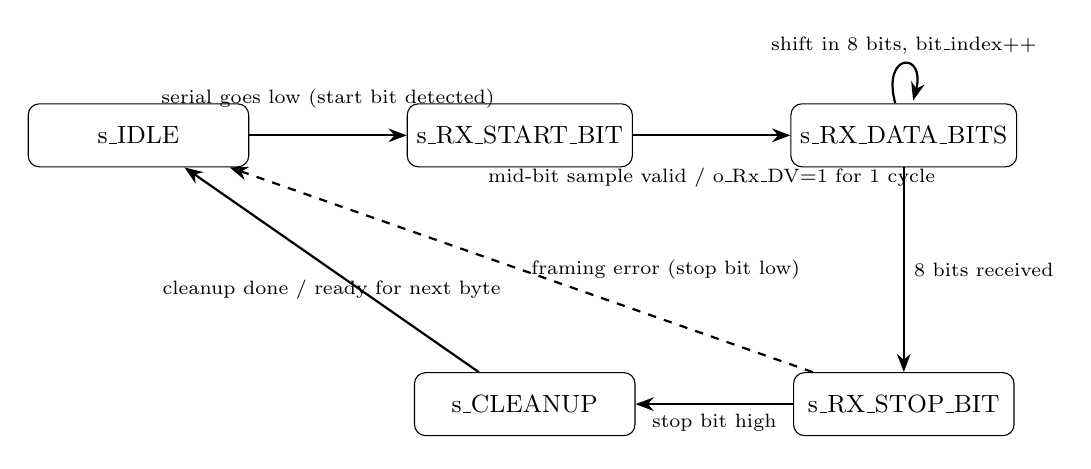
\begin{tikzpicture}[
    >=Stealth,
    node distance=26mm and 20mm,
    fsmstate/.style={draw, rounded corners, minimum width=28mm, minimum height=8mm, font=\small},
    fsmarrow/.style={->, thick},
    fsmdashed/.style={->, thick, dashed}
]

% --- States (two-row layout) ---
\node[fsmstate] (idle)  {s\_IDLE};
\node[fsmstate, right=of idle] (start) {s\_RX\_START\_BIT};
\node[fsmstate, right=of start] (data)  {s\_RX\_DATA\_BITS};

\node[fsmstate, below=of data] (stop)  {s\_RX\_STOP\_BIT};
\node[fsmstate, left=of stop] (clean) {s\_CLEANUP};

% --- Normal transitions ---
\draw[fsmarrow] (idle)  -- node[above ,yshift=6pt, font=\scriptsize]{serial goes low (start bit detected)} (start);

\draw[fsmarrow] (start) -- node[below,yshift=-8pt, font=\scriptsize]{mid-bit sample valid / o\_Rx\_DV=1 for 1 cycle} (data);

\draw[fsmarrow] (data)  edge[loop above] node[above, font=\scriptsize]{shift in 8 bits, bit\_index++} (data);

\draw[fsmarrow] (data)  -- node[right, font=\scriptsize]{8 bits received} (stop);

\draw[fsmarrow] (stop)  -- node[below, font=\scriptsize]{stop bit high} (clean);

\draw[fsmarrow] (clean) -- node[below, font=\scriptsize]{cleanup done / ready for next byte} (idle);

% --- Error path (framing error / invalid stop bit) ---
\draw[fsmdashed] (stop) edge node[right, font=\scriptsize]{framing error (stop bit low)} (idle);

\end{tikzpicture}
\caption{UART Receiver FSM (\texttt{uart\_rx.sv})}
\label{fig:uart_rx_fsm}
\end{figure}



% ============================================
% Implementation Results
% ============================================
\section{Implementation Results}

\subsection{Resource Utilization}

The FPGA resource utilization for the complete system is summarized in Figure \ref{fig:fitter_summary}. The design was successfully compiled and fitted to the Cyclone IV E EP4CE115F29C7 device.

\begin{figure}[H]
    \centering
    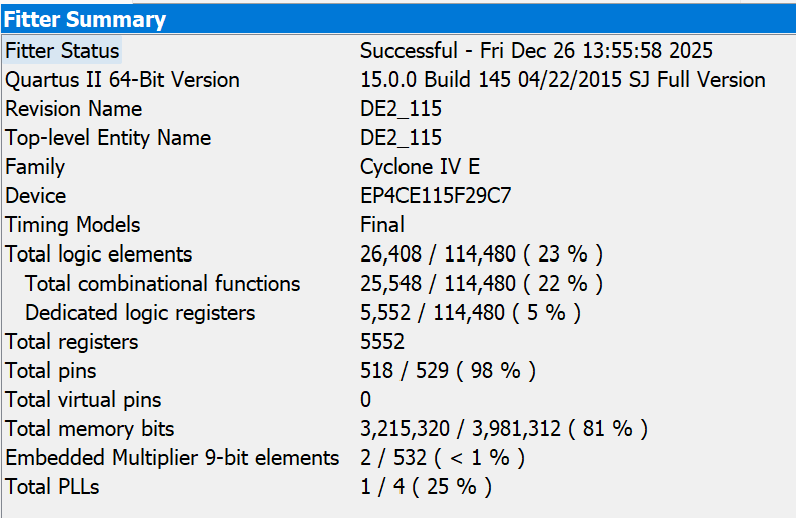
\includegraphics[width=0.95\textwidth]{fitter_summary.png}
    \caption{FPGA Fitter Summary - Resource Utilization}
    \label{fig:fitter_summary}
\end{figure}

The fitter summary reveals the following resource utilization:
\begin{itemize}
    \item \textbf{Logic Elements}: 26,408 out of 114,480 (23\%) - The design uses a moderate amount of combinational logic, with 25,548 combinational functions (22\%) and 5,552 dedicated logic registers (5\%).
    \item \textbf{Memory Bits}: 3,215,320 out of 3,981,312 (81\%) - High memory utilization reflects the extensive use of BRAM for sprite data, palettes, bounds information, and audio samples, as well as SRAM for background images.
    \item \textbf{Pins}: 518 out of 529 (98\%) - Nearly all available I/O pins are utilized for VGA output, audio codec interface, SRAM interface, UART communication, and control signals.
    \item \textbf{Embedded Multipliers}: 2 out of 532 (less than 1\%) - Minimal use of hardware multipliers, indicating that arithmetic operations are primarily implemented using logic elements.
    \item \textbf{PLLs}: 1 out of 4 (25\%) - One PLL is used to generate the 74.25MHz VGA clock from the 50MHz system clock.
\end{itemize}

The successful compilation and fitting demonstrate that the design fits within the available resources of the target FPGA device, with memory being the most constrained resource at 81\% utilization.

% ============================================
% Timing Analysis
% ============================================
\section{Timing Analysis}

\subsection{Overview}
Timing verification was performed using the Quartus Prime TimeQuest Timing Analyzer. The analysis evaluated the design's performance across multiple PVT (Process, Voltage, and Temperature) corners to ensure robust operation. The primary clock domains analyzed include the 50MHz system clock, the 74.25MHz VGA clock, the 12MHz audio clock, and the 100kHz I2C configuration clock.

\begin{figure}[H]
    \centering
    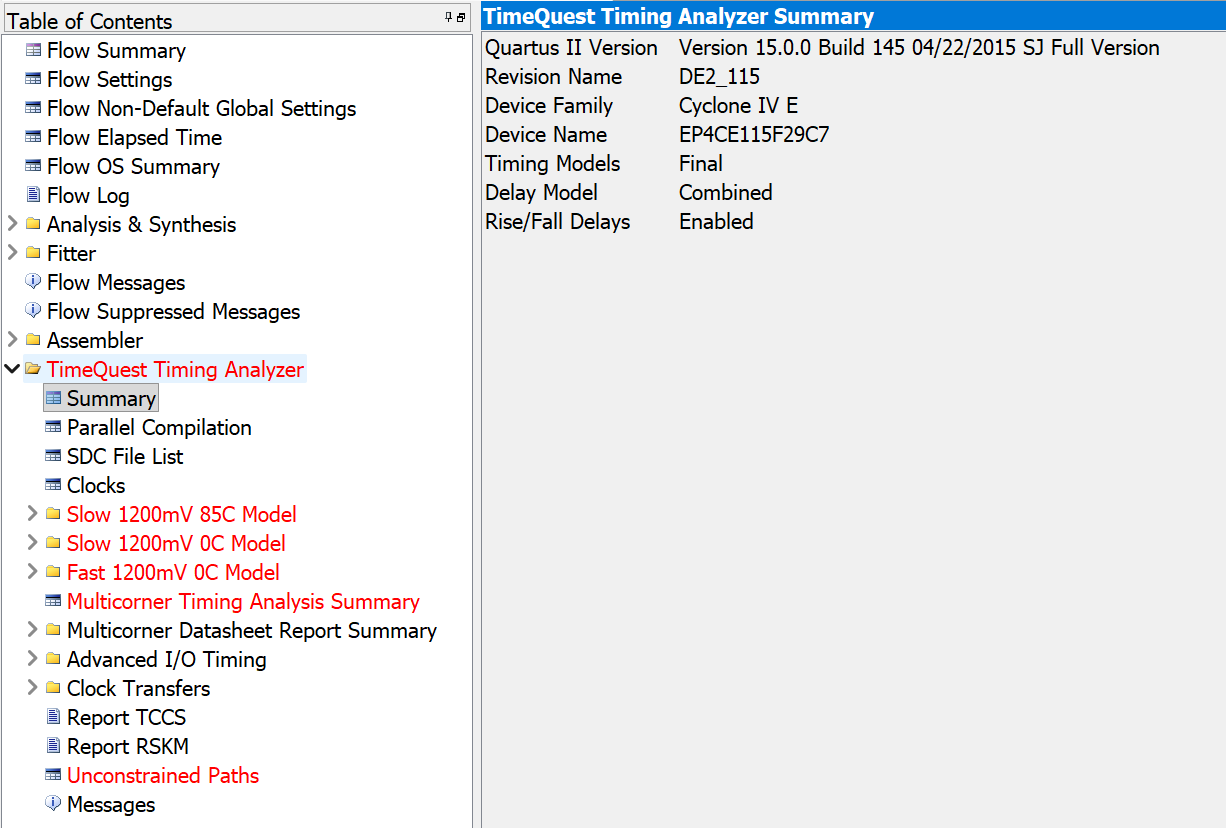
\includegraphics[width=0.95\textwidth]{timing_analyzer.png}
    \caption{TimeQuest Timing Analyzer Summary Interface}
    \label{fig:timing_analyzer}
\end{figure}

Figure \ref{fig:timing_analyzer} shows the TimeQuest Timing Analyzer interface, displaying the timing analysis summary for the Cyclone IV E device (EP4CE115F29C7). The analyzer provides comprehensive timing information across multiple corners and models, including the Slow 1200mV 85C and Fast 1200mV 0C models shown in the navigation tree.

\subsection{Worst-Case Setup Summary (Slow 1200mV 85C)}
The most critical timing results were observed in the \textbf{Slow 1200mV 85C} model, which represents the device's behavior under low voltage and high temperature conditions. As shown in Table \ref{tab:timing_setup}, significant setup time violations exist in the high-frequency domains.

\begin{table}[h]
\centering
\caption{Setup Summary: Slow 1200mV 85C Model}
\label{tab:timing_setup}
\begin{tabular}{|l|l|c|c|}
\hline
\textbf{Clock Label} & \textbf{Frequency} & \textbf{Worst-case Slack (ns)} & \textbf{Total Negative Slack (TNS)} \\ \hline
\texttt{CLOCK\_50} & 50.00 MHz & -74.285 & -1560.680 \\ \hline
\texttt{clk[1]} (VGA) & 74.25 MHz & -28.946 & -38199.688 \\ \hline
\texttt{clk[3]} (Audio) & 12.00 MHz & -7.774 & -2238.638 \\ \hline
\texttt{clk[2]} (I2C) & 100.00 kHz & 10.330 & 0.000 \\ \hline
\end{tabular}
\end{table}

\subsection{Multicorner Summary}
A summary of the timing performance across all corners is provided in Table \ref{tab:multicorner}. While the setup time fails in the slow corners, the hold time remains positive across all domains, indicating no race conditions were detected.

\begin{table}[h]
\centering
\caption{Multicorner Timing Analysis Summary}
\label{tab:multicorner}
\begin{tabular}{|l|c|c|c|c|}
\hline
\textbf{Clock} & \textbf{Setup Slack} & \textbf{Hold Slack} & \textbf{Recovery} & \textbf{Removal} \\ \hline
\textbf{Worst-case} & -74.285 & 0.140 & -2.228 & 0.398 \\ \hline
\texttt{CLOCK\_50} & -74.285 & 0.140 & -2.228 & 0.398 \\ \hline
\texttt{VGA (74.25 MHz)} & -28.946 & 0.140 & 8.296 & 2.065 \\ \hline
\texttt{Audio (12 MHz)} & -7.774 & 0.327 & N/A & N/A \\ \hline
\texttt{I2C (100 kHz)} & 10.330 & 0.182 & N/A & N/A \\ \hline
\end{tabular}
\end{table}

\subsection{Analysis and Impact}
The negative slack observed in the \texttt{CLOCK\_50} and \texttt{VGA} domains indicates that the current implementation exceeds the maximum theoretical frequency for the target FPGA under worst-case conditions. However, in laboratory environments (typically near 25C), the design remains operational. To resolve these violations for production-grade stability, future iterations would require pipelining the long combinatorial paths in the \texttt{VGA\_Image\_Overlay} and improving logic distribution within the \texttt{Position\_Controller}.

% ============================================
% Challenges and Solutions
% ============================================
\section{Challenges and Solutions}

Throughout the development of this FPGA-based zombie shooting game, we encountered numerous technical challenges that required innovative solutions and deep understanding of digital design principles. This section documents the major challenges faced and the solutions implemented to overcome them.

\subsection{VGA Timing Compensation}

\subsubsection{Challenge: BRAM and SRAM Read Latency in VGA Pipeline}
The VGA controller generates pixel coordinates, but both BRAM and SRAM has a 1-cycle read latency. If coordinates are output at cycle T, the corresponding pixel data arrives at cycle T+1, causing a one-pixel shift in the displayed image.

\subsubsection{Solution: Predictive Coordinate Generation}
We modified the VGA Controller to calculate and output pixel coordinates one cycle ahead of when they are actually needed. The module computes active coordinates based on the current counter values and registers them for the next cycle, ensuring that when pixel data arrives from BRAM, it corresponds to the correct screen position. This required careful analysis of the VGA timing parameters and precise coordination between the controller and compositor modules.

\subsection{Transparency Detection Optimization}

\subsubsection{Challenge: Efficient Transparency Detection for Zombie Sprites}
Detecting transparent pixels in zombie sprites is critical for proper rendering, but implementing this efficiently proved challenging. We needed a method that could quickly determine if a pixel position within a zombie sprite is transparent without incurring excessive latency or resource usage.

\subsubsection{Attempt 1: Sequential Pixel Index Checking}
Our initial approach was to check the pixel index for all zombies at the beginning of each frame. However, this method suffered from significant latency: with BRAM having a 1-cycle read delay and up to 20 zombies to check, this approach would require 20 cycles of sequential BRAM reads. This delay was unacceptable for real-time rendering at 60 FPS, as it would cause visible artifacts and timing violations in the rendering pipeline.

\subsubsection{Attempt 2: 2D Boolean Array Lookup}
To eliminate the sequential delay, we attempted to pre-compute a 2D boolean array \texttt{trans\_arr[x][y]} that records the transparent regions of each zombie sprite at initialization. During rendering, we would simply read \texttt{trans\_arr[x][y]} to determine if a pixel is transparent. However, this approach created a massive multiplexer: for a 102×149 pixel zombie sprite, accessing \texttt{trans\_arr[x][y]} required a 15,198-input MUX (102×149). This enormous combinational logic:
\begin{itemize}
    \item Caused extremely long synthesis and routing times
    \item Resulted in poor timing analysis with significant negative slack
    \item Consumed excessive logic resources
    \item Made the design impractical for implementation
\end{itemize}

\subsubsection{Solution: Pre-computed Column-Based Bounds in BRAM}
Our final solution uses a column-based bounds approach that balances efficiency and resource usage:
\begin{itemize}
    \item \textbf{Pre-computation}: For each zombie sprite, we pre-calculate transparency bounds for each X coordinate (column). The bounds store the minimum and maximum Y coordinates where non-transparent pixels exist in that column, encoded as a 16-bit value: [15:8] = Max Y, [7:0] = Min Y
    \item \textbf{BRAM Storage}: These bounds are stored in dedicated BRAM instances (one per zombie scale), with each address corresponding to an X coordinate
    \item \textbf{Efficient Lookup}: During rendering, we fetch bounds for up to 4 candidate zombies in parallel using dual-port BRAMs (2 BRAM instances per scale, fetching 2 bounds per instance). The bounds data arrives in Layer 2 of the pipeline
    \item \textbf{Quick Rejection}: For each candidate zombie, we check if the current Y coordinate falls within the bounds range. If Y is outside [Min Y, Max Y], the entire column is transparent at this position, and we can skip fetching the pixel data
    \item \textbf{Pixel-Level Check}: Only when Y is within bounds do we fetch the actual pixel index and check if it equals 0x00 (transparent)
\end{itemize}

This approach provides several advantages:
\begin{itemize}
    \item \textbf{Low Latency}: Bounds checking requires only 1 BRAM read cycle, and we can check up to 4 zombies in parallel
    \item \textbf{Resource Efficiency}: Each bounds BRAM stores only 102 entries (one per X coordinate) rather than 15,198 boolean values
    \item \textbf{Timing Friendly}: The bounds lookup uses simple BRAM access and comparison logic, avoiding the massive MUX structure
    \item \textbf{Memory Bandwidth Savings}: By rejecting transparent columns early, we avoid unnecessary pixel data fetches, reducing memory bandwidth by 60-70\%
\end{itemize}

The bounds-based approach successfully balances performance, resource usage, and timing closure, enabling real-time rendering of up to 20 zombies simultaneously while maintaining 60 FPS.

\subsection{Multi-Sprite Rendering Performance}

\subsubsection{Challenge: Rendering 20 Simultaneous Zombies}
Rendering up to 20 independent zombies with individual positions, scales, and states requires efficient candidate selection and bounds checking to avoid processing all zombies for every pixel.

\subsubsection{Solution: Candidate Selection and Bounds Optimization}
We implemented a two-stage optimization:
\begin{itemize}
    \item \textbf{Candidate Selection}: For each pixel, only zombies whose bounding boxes overlap the current position are considered (up to 4 candidates)
    \item \textbf{Pre-computed Bounds}: Transparency bounds are pre-calculated and stored in BRAM, allowing quick rejection of transparent columns without accessing sprite pixel data
    \item \textbf{Priority-Based Rendering}: Among overlapping sprites, the backmost (lowest Y coordinate) is rendered first, ensuring correct depth ordering
\end{itemize}

This approach reduces memory bandwidth by 80-90\% compared to naively checking all zombies for every pixel, enabling real-time rendering at 60 FPS.

\subsection{Memory Resource Constraints}

\subsubsection{Challenge: High Memory Utilization}
The system requires extensive memory for sprites, palettes, audio samples, and background images. With 81\% of available BRAM utilized, careful memory management was essential. The challenge was compounded by the need for multiple zombie scales (6 different sizes), each requiring separate sprite and bounds BRAM instances. Additionally, we encountered an SRAM capacity limitation when storing the start screen background image.

\subsubsection{Solution: Efficient Memory Architecture}
We optimized memory usage through several strategies:
\begin{itemize}
    \item \textbf{Indexed Color System}: Using 8-bit indexed color instead of 24-bit RGB reduced memory requirements by 66\% for sprite data
    \item \textbf{Shared Palettes}: A single palette is shared across all zombie scales, rather than duplicating palettes for each scale
    \item \textbf{Strategic Memory Allocation}: Large, infrequently accessed data (background images) stored in external SRAM; frequently accessed data (sprites, palettes) in on-chip BRAM
    \item \textbf{Dual-Port BRAM Utilization}: Using dual-port BRAMs for bounds data allows parallel fetching for multiple zombie candidates, reducing the number of required BRAM instances
    \item \textbf{SRAM Capacity Optimization}: When we encountered SRAM capacity limitations for the start screen background, we reduced the K-means clustering parameter from K=256 to K=64. This change reduced the color palette from 256 to 64 colors, allowing the start background to use 4-bit indices instead of 8-bit indices, effectively halving the memory requirement for the start screen image. While this slightly reduced color fidelity, the visual quality remained acceptable for the start screen, and the memory savings were critical for fitting all required images within the 2MB SRAM capacity
\end{itemize}

\subsection{IMU Data Processing and Drift Management}

\subsubsection{Challenge: Sensor Drift and Noise}
IMU sensors exhibit inherent drift due to integration of noise and bias errors. Without proper handling, the aim cursor would gradually drift across the screen even when the sensor is stationary, making the game unplayable.

\subsubsection{Solution: Calibration and Intelligent Drift Correction}
We implemented a comprehensive drift management system:
\begin{itemize}
    \item \textbf{Self-Calibration Phase}: Upon startup, the system collects 2,048 samples over 10 seconds to calculate sensor bias and gravity offset
    \item \textbf{Deadzone Threshold}: Small accelerations below a threshold are ignored, preventing micro-movements from accumulating
    \item \textbf{Smart Reset Timer}: If the sensor remains stable (within deadzone) for 0.2 seconds, velocity accumulators are automatically zeroed, implementing a "leaky integrator" behavior
    \item \textbf{High-Precision Accumulators}: Using 64-bit internal registers for velocity integration minimizes quantization errors
\end{itemize}

This approach provides stable, responsive control while automatically correcting for drift without requiring manual recalibration.

% ============================================
% Experience of the Project
% ============================================
\section{Experience of the Project}

This project provided an invaluable opportunity to apply digital design principles to create a complex, real-time interactive system. The experience encompassed system-level architecture design, low-level hardware optimization, and integration of multiple heterogeneous subsystems.

\subsection{Technical Learning Outcomes}

\subsubsection{System-Level Design}
Working on this project deepened our understanding of system-on-chip (SoC) design principles. We learned to:
\begin{itemize}
    \item Design modular architectures with clear interfaces between subsystems
    \item Balance performance, resource utilization, and design complexity
    \item Make architectural decisions considering timing, area, and power constraints
    \item Integrate multiple clock domains safely and efficiently
\end{itemize}

\subsubsection{Memory System Design}
The project provided hands-on experience with hierarchical memory architectures:
\begin{itemize}
    \item Understanding the trade-offs between SRAM (large capacity, higher latency) and BRAM (fast access, limited capacity)
    \item Implementing efficient memory access patterns to maximize bandwidth
    \item Using indexed color systems and palettes to optimize memory usage
    \item Managing memory resources when approaching device limits (81\% utilization)
\end{itemize}

\subsubsection{Pipeline Design and Timing}
We gained practical experience with:
\begin{itemize}
    \item Designing multi-stage pipelines to handle memory latencies
    \item Timing closure challenges and optimization techniques
    \item Balancing pipeline depth with resource utilization
    \item Compensating for different memory access latencies in a unified pipeline
\end{itemize}

\subsubsection{Real-Time System Constraints}
The project required meeting strict real-time constraints:
\begin{itemize}
    \item Maintaining 60 FPS rendering at 1280x720 resolution
    \item Ensuring deterministic timing for game mechanics
    \item Handling multiple parallel operations (rendering, audio, input processing) without interference
    \item Debugging timing-sensitive issues that only appear under specific conditions
\end{itemize}

\subsection{Problem-Solving Skills}

The project presented numerous challenges that required creative problem-solving:
\begin{itemize}
    \item \textbf{Debugging Complex Systems}: Identifying issues in a system with multiple interacting subsystems required systematic debugging approaches, including signal tracing, simulation, and hardware testing
    \item \textbf{Performance Optimization}: Balancing code clarity with performance requirements, and making informed trade-offs between different optimization strategies
    \item \textbf{Resource Management}: Working within FPGA resource constraints required careful planning and optimization at every level
    \item \textbf{Integration Challenges}: Integrating subsystems developed independently required careful attention to interfaces, timing, and synchronization
\end{itemize}

\subsection{FPGA Development Workflow}

We gained proficiency in the complete FPGA development workflow:
\begin{itemize}
    \item \textbf{Design Entry}: Writing SystemVerilog code following best practices and coding standards
    \item \textbf{Simulation}: Using ModelSim for functional verification before hardware deployment
    \item \textbf{Synthesis and Implementation}: Using Quartus Prime for synthesis, place-and-route, and timing analysis
    \item \textbf{Debugging Tools}: Utilizing SignalTap Logic Analyzer, timing analyzer, and resource utilization reports
    \item \textbf{Iterative Development}: Refining designs based on timing analysis, resource reports, and hardware testing
\end{itemize}

\subsection{Interdisciplinary Integration}

The project required integrating knowledge from multiple domains:
\begin{itemize}
    \item \textbf{Digital Design}: State machines, pipelines, memory interfaces
    \item \textbf{Computer Graphics}: Image compositing, transparency, sprite rendering
    \item \textbf{Signal Processing}: Audio playback, sensor data filtering
    \item \textbf{Embedded Systems}: UART communication, I2C protocol, GPIO interfacing
    \item \textbf{Game Design}: Collision detection, difficulty scaling, state management
\end{itemize}

This interdisciplinary approach mirrors real-world engineering projects where multiple technical domains must be integrated into a cohesive system.

\subsection{Project Management and Teamwork}

Working on a project of this complexity required:
\begin{itemize}
    \item \textbf{Task Decomposition}: Breaking the project into manageable modules that could be developed in parallel
    \item \textbf{Version Control}: Managing code changes across multiple team members
    \item \textbf{Documentation}: Maintaining clear documentation for interfaces and design decisions
    \item \textbf{Testing Strategy}: Developing systematic approaches to test individual modules and integrated systems
\end{itemize}

\subsection{Real-World Application Insights}

This project provided insights into how complex systems are built in industry:
\begin{itemize}
    \item \textbf{Performance vs. Resources}: Real-world designs always involve trade-offs between performance, resource usage, and development time
    \item \textbf{Timing Closure}: Meeting timing requirements is often one of the most challenging aspects of FPGA design
    \item \textbf{Modularity}: Well-designed interfaces and modular architectures are essential for managing complexity
    \item \textbf{Iterative Refinement}: Complex systems rarely work correctly on the first attempt; iteration and refinement are essential
\end{itemize}

\subsection{Challenges and Growth}

The project presented significant challenges that contributed to our growth as digital designers:
\begin{itemize}
    \item \textbf{Persistence}: Debugging timing issues and integration problems required patience and systematic approaches
    \item \textbf{Attention to Detail}: Small errors in timing or synchronization could cause subtle bugs that were difficult to identify
    \item \textbf{System Thinking}: Understanding how changes in one subsystem affect others required thinking at the system level
    \item \textbf{Documentation Discipline}: Maintaining clear documentation became essential as the project complexity grew
\end{itemize}

\subsection{Conclusion}

This project successfully demonstrated that complex, interactive multimedia applications can be efficiently implemented on FPGA platforms. The experience provided practical skills in digital design, system integration, and real-time system development that are directly applicable to industry projects. The challenges encountered and overcome during development have significantly enhanced our understanding of FPGA design principles and system-level engineering.

The project serves as a comprehensive example of modern FPGA system design, integrating graphics rendering, audio processing, sensor interfacing, and game logic into a cohesive, real-time interactive system. The lessons learned and skills developed through this project will be valuable in future digital design endeavors.

% ============================================
% Appendices
% ============================================
\newpage
\appendix

\section{Project Resources}

This section provides links to additional project resources including source code and demonstration videos.

\subsection{GitHub Repository}

The complete source code, documentation, and project files are available in the GitHub repository:

\url{https://github.com/jasonpan0930/NTU_DCLAB/tree/main/final}

The repository contains:
\begin{itemize}
    \item Complete SystemVerilog source code for all modules
    \item BRAM memory initialization files
    \item Quartus project configuration files
    \item Image processing scripts for K-means color quantization
    \item Project documentation and README files
\end{itemize}

\subsection{Demo Video}

A demonstration video showcasing the game in action is available at:

\url{https://drive.google.com/file/d/1JyUkKLRqYuORODn6-K4xCcDV3Nc670AX/view?usp=drive_link}

The video demonstrates:
\begin{itemize}
    \item Real-time gameplay with IMU-based aiming control
    \item Multi-zombie rendering and collision detection
    \item Audio playback and sound effects
    \item Game state transitions and difficulty scaling
    \item Visual effects including sprite scaling and hit detection
\end{itemize}

\end{document}